%!TEX TS-program = pdflatex
%!TEX root = ../main.tex
%!TEX encoding = UTF-8 Unicode


\section{Conclusions}
\label{section:conclusions}

Considering the overall results shown in \autoref{fig:graph}, the optimal approach for optimising the efficiency of queries 1 (Export/import revenue value) and 2 (Late delivery) might be to use the materialized views proposed in \autoref{section:materialization} but this happens to be the worst-case scenario for query 3 (Returned item loss).
The opposite situation occurs when using the indexes defined in \autoref{sec:indexes}: the query 3 is optimised, but queries 1 and 2 show roughly the same run times as the na\"{i}ve solution.

Assuming that all the three queries have the same importance (i.e., none of them is being executed a lot more frequently than the others), a good trade-off may seem to use \textit{materialized views} and \textit{indexes} (\autoref{subsection:indexes_mv}). This solution, by the way, does not meet the size constraint of the project.

The final solution that is being proposed for the given problem concerns using the (\textit{vertical}) \textit{fragmentation} reported in \autoref{sec:fragmentation} without any additional index. Query 1 is executed in \SI{15.84}{\s}, i.e.\ 2.5 times faster than the na\"{i}ve solution; query 2 runs in \SI{20.36}{\s}, i.e.\ it is 2.3 times faster than the related na\"{i}ve solution; query 3 is executed in \SI{2.29}{\s}, i.e.\ 3.5 times faster than the corresponding na\"{i}ve solution.


\begin{figure}[h]
\centering
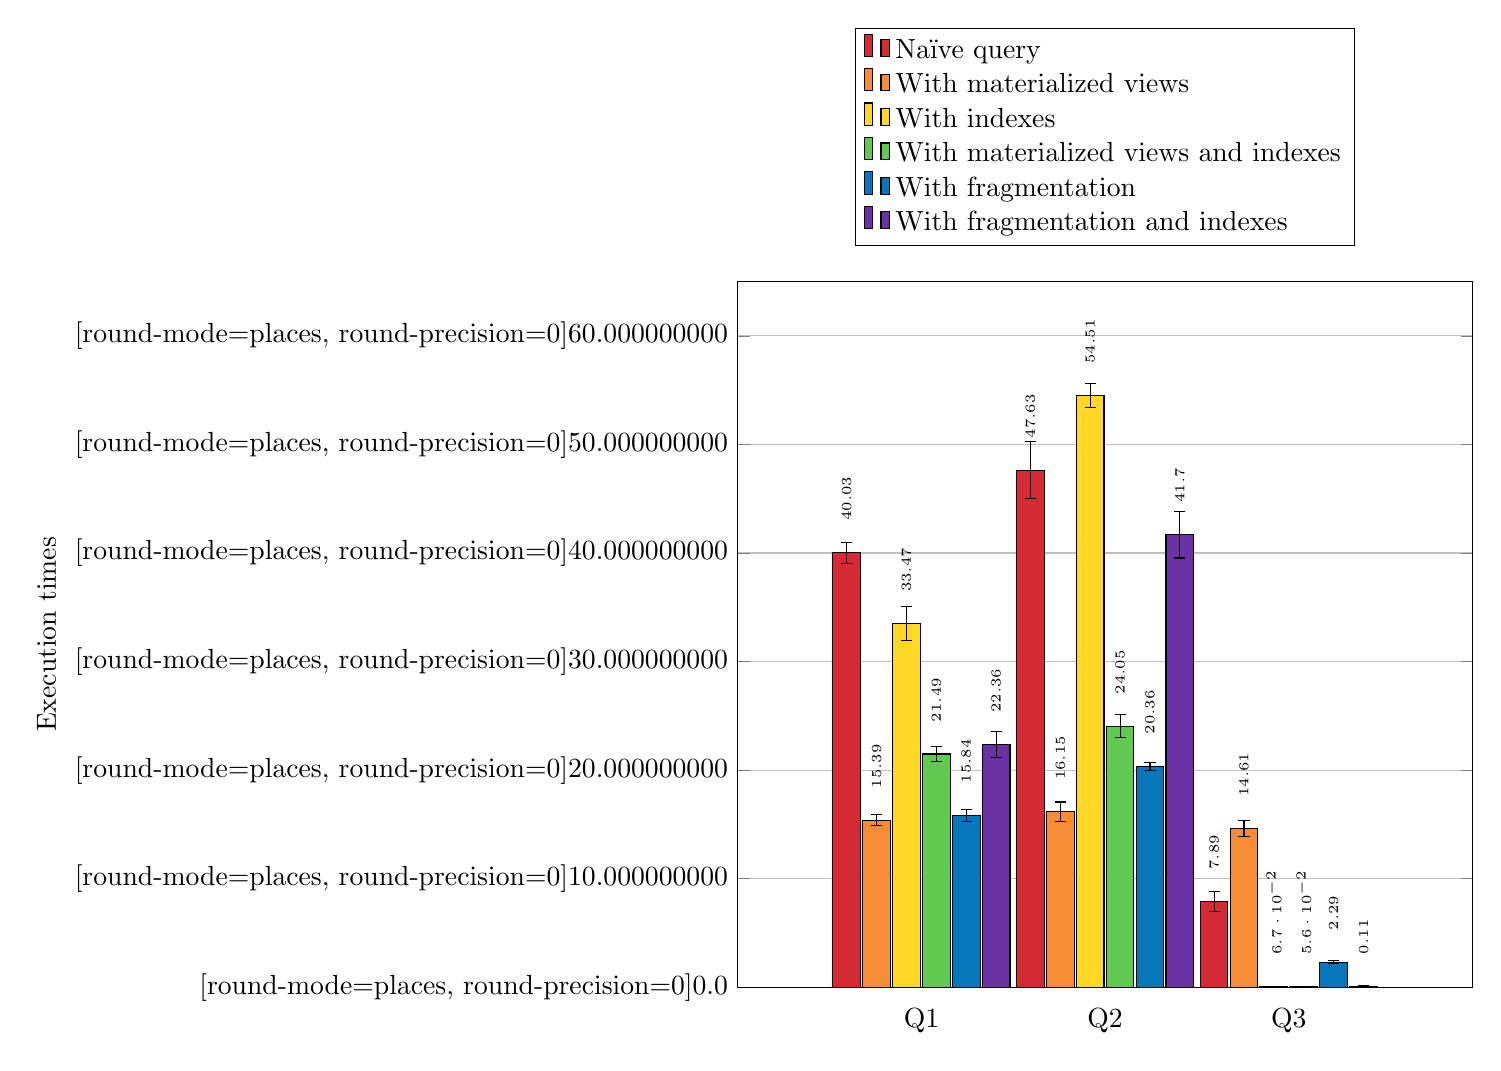
\begin{tikzpicture}

	\definecolor{Red}{RGB}{212, 42, 52}
	\definecolor{Orange}{RGB}{247, 140, 55}
	\definecolor{Yellow}{RGB}{255, 216, 39}
	\definecolor{Apple}{RGB}{98, 202, 80}
	\definecolor{Blue}{RGB}{6, 119, 186}
	\definecolor{Grape}{RGB}{106, 50, 165}

      \begin{axis}[
      width=.9\textwidth,
      height=30em,
      major x tick style = transparent,
      ybar=2*\pgflinewidth,
      %bar width=25pt,
      ylabel={Execution times},
      ymajorgrids = true,
      symbolic x coords={Q1,Q2,Q3},
      xtick = data,
      scaled y ticks = true,
      yticklabel={\SI[round-mode=places, round-precision=0]{\tick}{\s}},
      enlarge x limits=.5,
      ymin=0, ymax=65,
      legend cell align=left,
      legend style={at={(0.5,1.05)},anchor=south},
      nodes near coords,
      every node near coord/.append style={yshift=.8em,anchor=south,font=\tiny,rotate=90, anchor=west},
  ]
      \addplot[style={fill=Red},error bars/.cd, y dir=both, y explicit]
          coordinates {
          (Q1,40.029) += (0,.971) -= (0,.971)
          (Q2,47.626) += (0,2.626) -= (0,2.626)
          (Q3,7.893) += (0,.915) -= (0,.915)};

      \addplot[style={fill=Orange},error bars/.cd, y dir=both, y explicit]
           coordinates {
           (Q1,15.392) += (0,.483) -= (0,.483)
           (Q2,16.153) += (0,.910) -= (0,.910)
          (Q3,14.608) += (0,.732) -= (0,.732)};

      \addplot[style={fill=Yellow},error bars/.cd, y dir=both, y explicit]
           coordinates {
           (Q1,33.472) += (0,1.556) -= (0,1.556)
           (Q2,54.506) += (0,1.100) -= (0,1.100)
           (Q3,0.067) += (0,0.025) -= (0,0.025)};

      \addplot[style={fill=Apple},error bars/.cd, y dir=both, y explicit]
           coordinates {
           (Q1,21.486) += (0,0.658) -= (0,0.658)
           (Q2,24.052) += (0,1.069) -= (0,1.069)
           (Q3,0.056) += (0,0.018) -= (0,0.018)};

      \addplot[style={fill=Blue},error bars/.cd, y dir=both, y explicit]
           coordinates {
           (Q1,15.839) += (0,0.558) -= (0,0.558)
           (Q2,20.360) += (0,0.380) -= (0,0.380)
           (Q3,2.294) += (0,0.147) -= (0,0.147)};

      \addplot[style={fill=Grape},error bars/.cd, y dir=both, y explicit]
           coordinates {
           (Q1,22.355) += (0,1.201) -= (0,1.201)
           (Q2,41.695) += (0,2.154) -= (0,2.154)
           (Q3,0.106) += (0,0.046) -= (0,0.046)};

      \legend{Na\"{i}ve query, With materialized views, With indexes, With materialized views and indexes, With fragmentation, With fragmentation and indexes}
  \end{axis}
  \end{tikzpicture}
  \caption{Query timings}
  \label{fig:graph}
\end{figure}